\documentclass[aspectratio=169,11pt]{beamer}

\usepackage{fontspec}
\usepackage{microtype}
\usepackage{tikz}

% Use Times New Roman when installed; otherwise use its metrically compatible
% open-source substitute available in the build environment.
\IfFontExistsTF{Times New Roman}{
  \setmainfont{Times New Roman}
}{
  \setmainfont{NimbusRoman-Regular.otf}[
    BoldFont=NimbusRoman-Bold.otf,
    ItalicFont=NimbusRoman-Italic.otf,
    BoldItalicFont=NimbusRoman-BoldItalic.otf
  ]
}
% TeX Gyre Heros ships with TeX Live and keeps Beamer's incidental sans-serif
% text portable without relying on separately installed Nimbus Sans files.
\setsansfont{texgyreheros-regular.otf}[
  BoldFont=texgyreheros-bold.otf,
  ItalicFont=texgyreheros-italic.otf,
  BoldItalicFont=texgyreheros-bolditalic.otf
]
\DeclareMathSizes{21}{21}{14.7}{10.95}
\usefonttheme{serif}
\setbeameroption{hide notes}

\definecolor{Ink}{HTML}{111111}
\definecolor{Navy}{HTML}{123B5D}
\definecolor{Muted}{HTML}{5D6268}
\definecolor{RuleGray}{HTML}{D8DCE0}
\definecolor{Placeholder}{HTML}{F5F6F7}
\definecolor{HighlightYellow}{HTML}{F3DA77}

\setbeamercolor{normal text}{fg=Ink,bg=white}
\setbeamercolor{structure}{fg=Navy}
\setbeamercolor{frametitle}{fg=Ink,bg=white}
\setbeamercolor{footline}{fg=Muted,bg=white}

\setbeamertemplate{navigation symbols}{}
\setbeamertemplate{headline}{}
\setbeamertemplate{frametitle}{
  \vspace{0.25cm}
  \parbox{0.9\textwidth}{\raggedright\hyphenpenalty=10000\exhyphenpenalty=10000\insertframetitle}\par
  \vspace{0.12cm}
  {\color{Navy}\rule{\textwidth}{0.65pt}\par}
  \vspace{0.1cm}
}
\setbeamertemplate{footline}{
  \begin{beamercolorbox}[wd=\paperwidth,ht=0.52cm,dp=0.22cm,leftskip=0.85cm,rightskip=0.85cm]{footline}
    {\color{Navy}\rule{1.15cm}{0.6pt}}\hspace{0.18cm}
    \fontsize{7.2}{8.5}\selectfont ENVR2002D · CLASS 9
    \hfill
    \textcolor{Navy}{\insertframenumber}
  \end{beamercolorbox}
}

\setbeamerfont{frametitle}{size=\fontsize{21}{24},series=\bfseries}
\setbeamerfont{normal text}{size=\fontsize{14}{18}}
\setbeamersize{text margin left=0.85cm,text margin right=0.85cm}
\setbeamertemplate{itemize item}{\raisebox{0.12ex}{\color{Navy}\small\textbullet}}

\newcommand{\partlabel}[1]{%
  {\color{Navy}\fontsize{9}{11}\selectfont\bfseries\MakeUppercase{#1}\par}
}

\begin{document}

% Slide 1 — lecture cover
\begin{frame}[plain]
  \vspace{0.55cm}
  \partlabel{ENVR2002D · Class 9}
  \vspace{0.2cm}
  {\color{Navy}\rule{\textwidth}{0.8pt}\par}

  \vspace{0.5cm}
  {\color{Ink}\fontsize{29}{33}\selectfont\bfseries
    How Can Science Support\\
    Maritime Decarbonisation?
  \par}

  \vspace{0.5cm}
  {\color{Ink}\fontsize{15}{20}\selectfont
    My journey from shipping to research, policy\\
    and implementation
  \par}

  \vfill
  {\color{Ink}\fontsize{11.2}{14}\selectfont\bfseries
    Jeremy Jiajing Chen, Year 4 PhD Candidate\\
    Division of Environment and Sustainability
  \par}
  \vspace{0.06cm}
  {\color{Muted}\fontsize{10}{12}\selectfont Hong Kong University of Science and Technology\par}
  \vspace{0.4cm}
  \note{
    [Sources]\par
    - Course and presenter: ENVR2002D course context supplied by Jeremy.\par
    - Lecture framing: approved two-part lecture plan.
  }
\end{frame}

% Slide 2 — session structure
\begin{frame}{Today’s lecture has two parts}
  \vspace{0.22cm}
  \begin{columns}[T,onlytextwidth]
    \begin{column}{0.46\textwidth}
      \partlabel{Part 1}
      \vspace{0.22cm}
      {\color{Ink}\fontsize{16}{19}\selectfont\bfseries
        How I ended up in shipping research
      \par}
      \vspace{0.13cm}
      {\color{Navy}\fontsize{10.5}{13}\selectfont\bfseries 30–40 minutes\par}
      \vspace{0.34cm}
      {\color{Ink}\fontsize{11.5}{15.5}\selectfont
        My shipping background, an unexpected PhD decision, my interest in
        computers and coding, and the research I do today.
      \par}
    \end{column}

    \begin{column}{0.04\textwidth}
      \centering
      {\color{RuleGray}\rule{0.6pt}{3.45cm}}
    \end{column}

    \begin{column}{0.46\textwidth}
      \partlabel{Part 2}
      \vspace{0.22cm}
      {\color{Ink}\fontsize{16}{19}\selectfont\bfseries
        How science supports maritime decarbonisation
      \par}
      \vspace{0.13cm}
      {\color{Navy}\fontsize{10.5}{13}\selectfont\bfseries 40 minutes\par}
      \vspace{0.34cm}
      {\color{Ink}\fontsize{11.5}{15.5}\selectfont
        How evidence helps us measure emissions, compare possible pathways,
        and move promising ideas towards implementation.
      \par}
    \end{column}
  \end{columns}

  \vfill
  {\color{Muted}\fontsize{8.5}{10.5}\selectfont
    Break between the two parts · Part 2 begins around 11:00
  \par}
  \note{
    [Sources]\par
    - Timing: course guidance supplied privately by Jeremy.\par
    - Content: approved Part 1 and Part 2 structure.
  }
\end{frame}

% Slide 3 — Part 1 divider
\begin{frame}[plain]
  \vfill
  \partlabel{Part 1}
  \vspace{0.3cm}
  {\color{Navy}\rule{1.3cm}{0.9pt}\par}

  \vspace{0.52cm}
  {\color{Ink}\fontsize{30}{34}\selectfont\bfseries
    How I ended up in\\
    shipping research
  \par}

  \vspace{0.48cm}
  {\color{Ink}\fontsize{14}{18.5}\selectfont
    My journey through family, shipping, computers\\
    and one unexpected decision.
  \par}
  \vfill
  \note{
    [Sources]\par
    - Personal narrative supplied by Jeremy.
  }
\end{frame}

% Slide 4 — shipping background
\begin{frame}{Shipping came before research.}
  \vspace{0.08cm}
  \begin{columns}[T,onlytextwidth]
    \begin{column}{0.58\textwidth}
      {\color{Ink}\fontsize{13.5}{18.5}\selectfont
        My grandfather and father both worked at sea, so shipping had always
        felt personal to me.
      \par}

      \vspace{0.5cm}
      {\color{Ink}\fontsize{13}{18}\selectfont
        I later studied \textbf{International Shipping Management}, followed
        by \textbf{Logistics and Environmental Policy}—first learning how the
        industry works, and then asking how it could change.
      \par}
    \end{column}

    \begin{column}{0.35\textwidth}
      \centering
      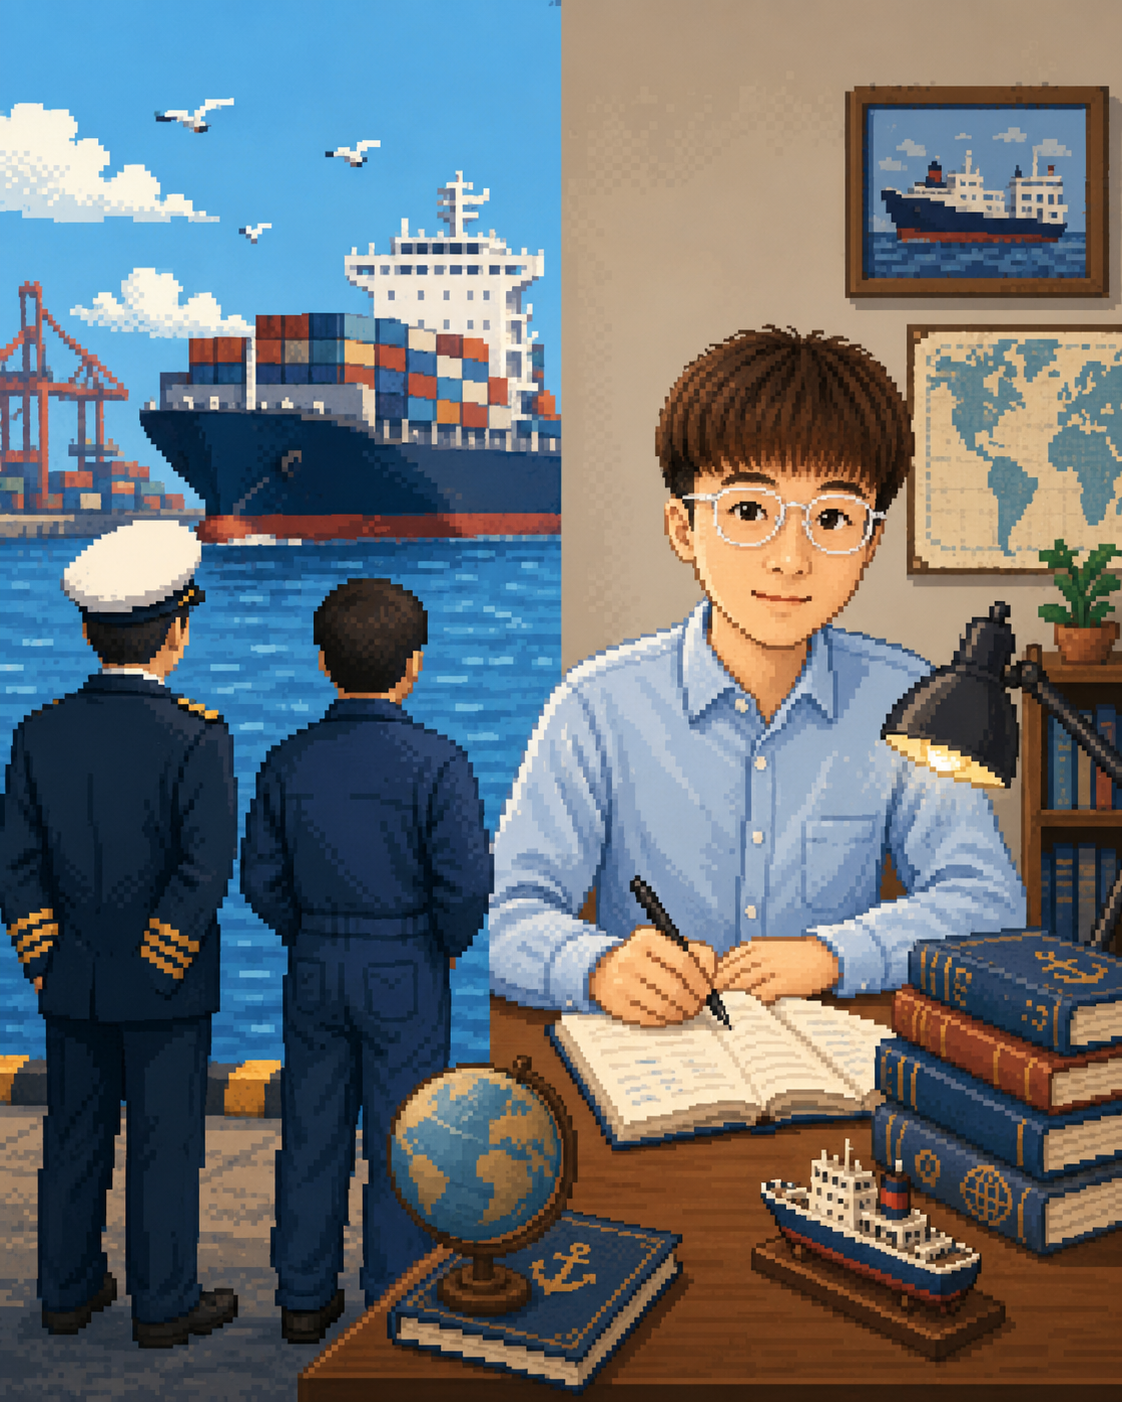
\includegraphics[
        width=0.93\linewidth,
        height=5.1cm,
        keepaspectratio
      ]{../assets/slide-4.png}
    \end{column}
  \end{columns}
  \note{
    [Sources]\par
    - Family and education background supplied by Jeremy.\par
    - Public cross-check: https://amoylimee.github.io/index.html\par
    - Visual: user-supplied pixel-art illustration, assets/slide-4.png.
  }
\end{frame}

% Slide 5 — PhD decision
\begin{frame}{A PhD was not my first choice.}
  \vspace{0.12cm}
  \begin{columns}[T,onlytextwidth]
    \begin{column}{0.58\textwidth}
      {\color{Ink}\fontsize{12.6}{17.5}\selectfont
        After my Master’s, I received an offer for a supply-chain management
        role at \textbf{Huawei}.
      \par}

      \vspace{0.35cm}
      {\color{Ink}\fontsize{12.6}{17.5}\selectfont
        I then applied for a short Research Assistant position, mainly to help
        pay for my flight home.
      \par}

      \vspace{0.35cm}
      {\color{Ink}\fontsize{12.6}{17.5}\selectfont
        A ten-minute conversation with Prof. Alexis Lau
        \textbf{(my supervisor)}
        changed the direction. The next day, I decided to pursue a PhD.
      \par}
    \end{column}

    \begin{column}{0.35\textwidth}
      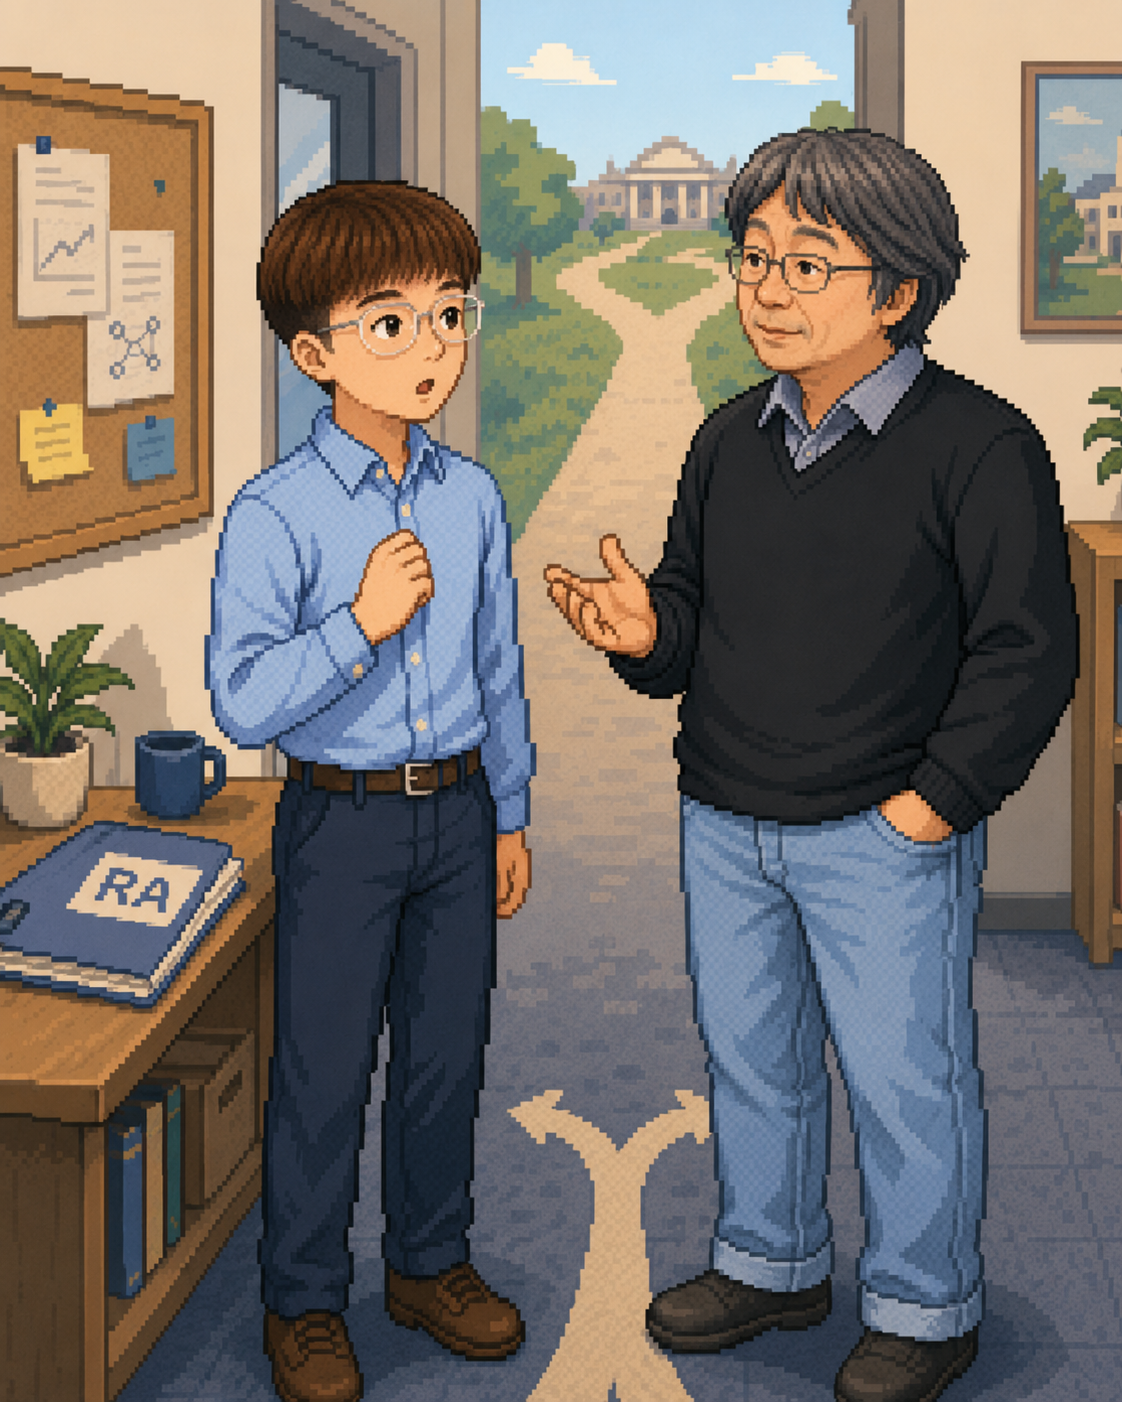
\includegraphics[
        width=0.93\linewidth,
        height=5.1cm,
        keepaspectratio
      ]{../assets/slide-5.png}
    \end{column}
  \end{columns}
  \note{
    [Sources]\par
    - Career and PhD-decision story: Jeremy's earlier presentation and
      personal account supplied privately.\par
    - Visual: user-supplied illustrative turning-point graphic,
      assets/slide-5.png.
  }
\end{frame}

% Slide 6 — computers and coding
\begin{frame}{I simply enjoyed computer games and coding.}
  \vspace{0.22cm}
  \begin{columns}[T,onlytextwidth]
    \begin{column}{0.58\textwidth}
      {\color{Ink}\fontsize{13.5}{18.5}\selectfont
        There was no deeper reason at the beginning: I liked spending time on
        a computer, playing games and writing code.
      \par}

      \vspace{0.5cm}
      {\color{Ink}\fontsize{13}{18}\selectfont
        Research gave me a way to bring these interests into my daily work:
        working with data, building algorithms and solving difficult problems.
      \par}
    \end{column}

    \begin{column}{0.35\textwidth}
      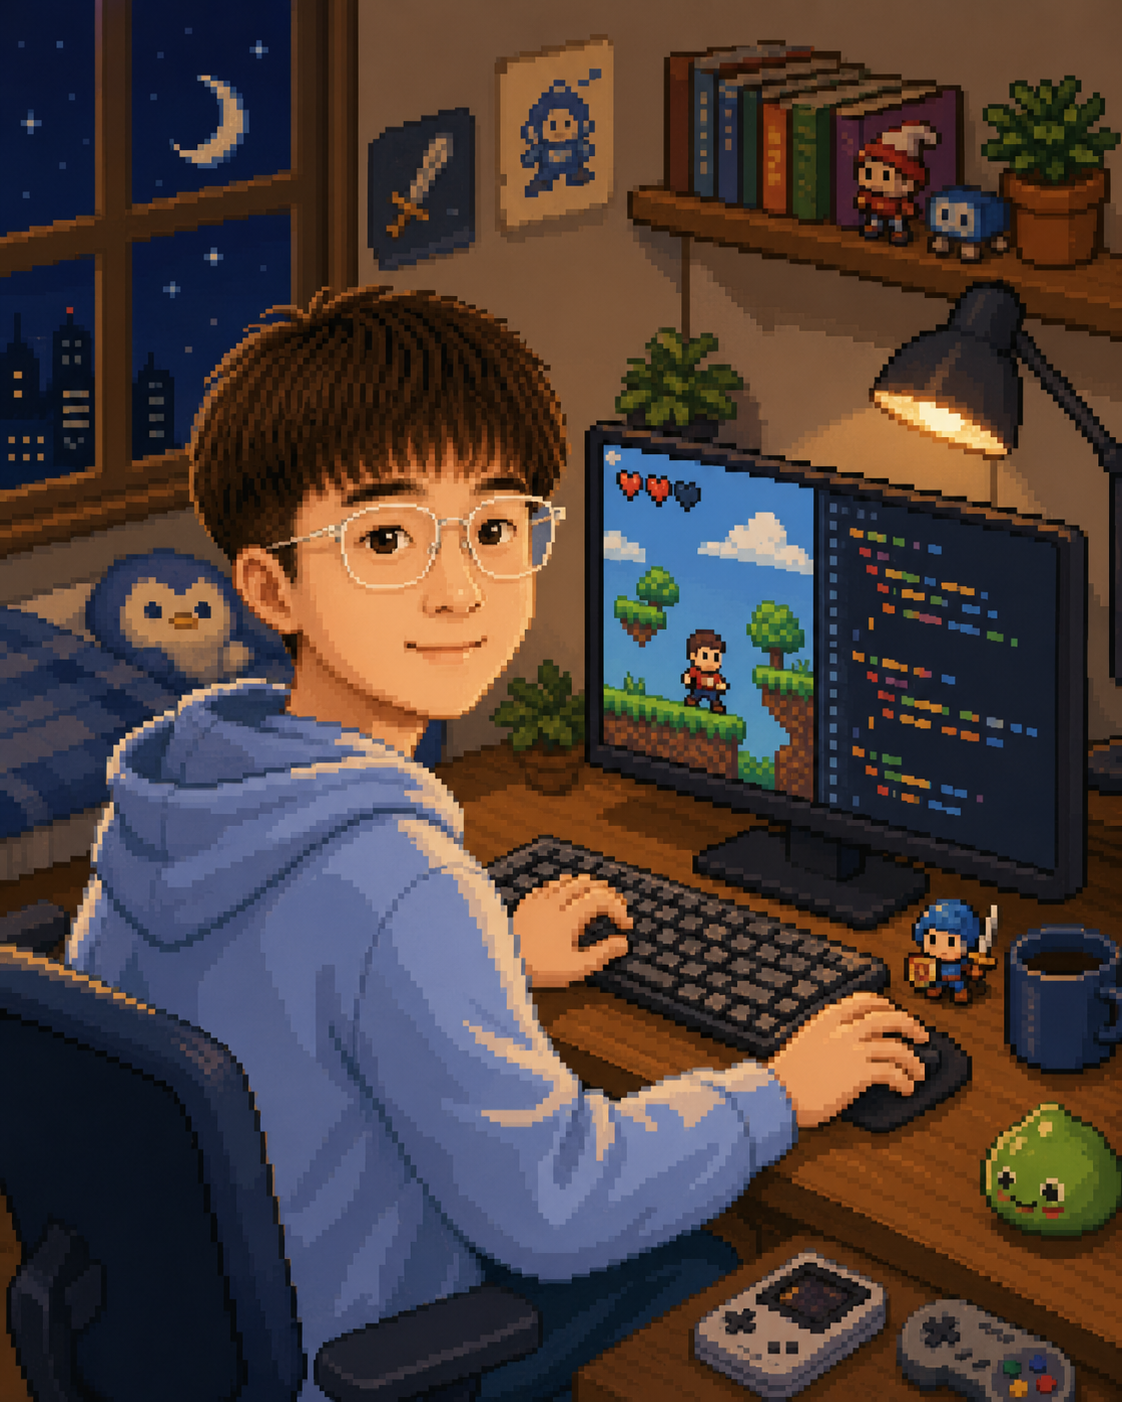
\includegraphics[
        width=0.93\linewidth,
        height=5.1cm,
        keepaspectratio
      ]{../assets/slide-6.png}
    \end{column}
  \end{columns}
  \note{
    [Sources]\par
    - Personal interest in computer games and coding supplied by Jeremy.\par
    - Research description cross-checked against Jeremy's public website.\par
    - Visual: user-supplied illustrative coding graphic,
      assets/slide-6.png.
  }
\end{frame}

% Slide 7 — current research
\begin{frame}{Today, I use data to understand how shipping works.}
  \vspace{0.08cm}
  \begin{columns}[T,onlytextwidth]
    \begin{column}{0.58\textwidth}
      {\color{Ink}\fontsize{13.2}{18}\selectfont
        From the shore, we see individual ships.
      \par}

      \vspace{0.48cm}
      {\color{Ink}\fontsize{13.2}{18}\selectfont
        In the data, we begin to see the whole system: where vessels move,
        where activity concentrates and where environmental impacts may occur.
      \par}
    \end{column}

    \begin{column}{0.35\textwidth}
      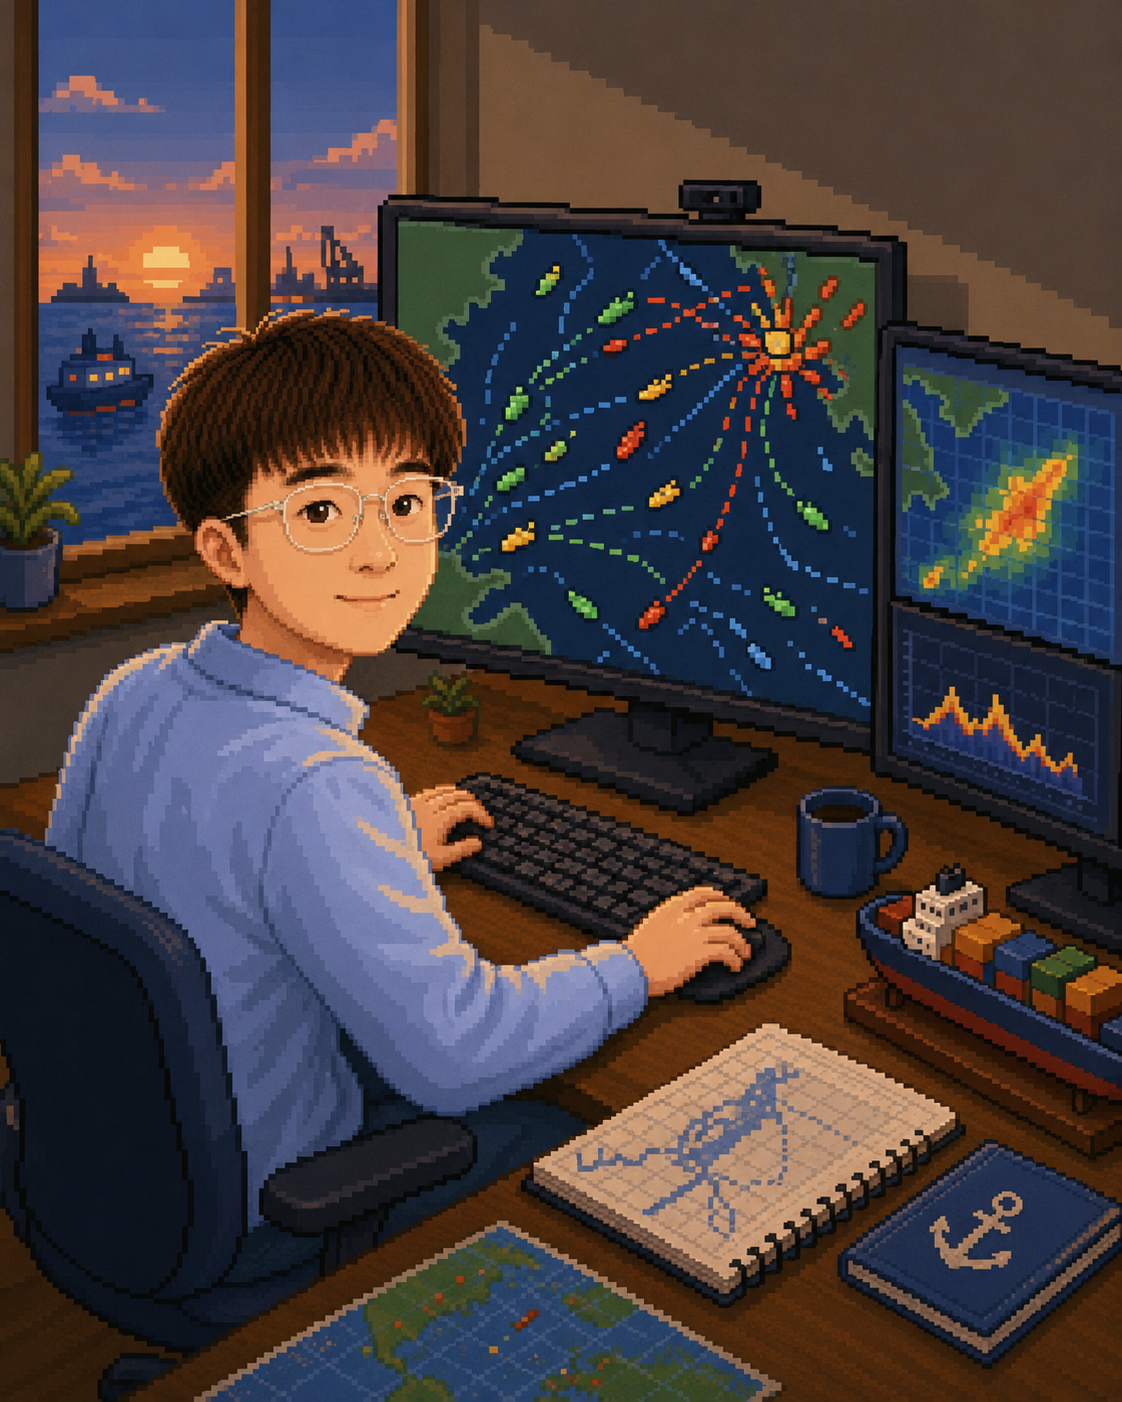
\includegraphics[
        width=0.93\linewidth,
        height=5.1cm,
        keepaspectratio
      ]{../assets/slide8.png}
    \end{column}
  \end{columns}
  \note{
    [Sources]\par
    - Research description cross-checked against Jeremy's public website.\par
    - Visual: user-supplied illustrative vessel-activity graphic,
      assets/slide8.png.
  }
\end{frame}

% Slide 8 — research logic
\begin{frame}{The methods are complicated. The logic is simple.}
  \vspace{0.55cm}
  \begin{columns}[c,onlytextwidth]
    \begin{column}{0.27\textwidth}
      \partlabel{Step 1}
      \vspace{0.22cm}
      {\color{Ink}\fontsize{16}{20}\selectfont\bfseries
        Observe real activity
      \par}
    \end{column}

    \begin{column}{0.07\textwidth}
      \centering
      {\color{Navy}\fontsize{18}{20}\selectfont →}
    \end{column}

    \begin{column}{0.27\textwidth}
      \partlabel{Step 2}
      \vspace{0.22cm}
      {\color{Ink}\fontsize{16}{20}\selectfont\bfseries
        Interpret it with code
      \par}
    \end{column}

    \begin{column}{0.07\textwidth}
      \centering
      {\color{Navy}\fontsize{18}{20}\selectfont →}
    \end{column}

    \begin{column}{0.27\textwidth}
      \partlabel{Step 3}
      \vspace{0.22cm}
      {\color{Ink}\fontsize{16}{20}\selectfont\bfseries
        Turn it into useful evidence
      \par}
    \end{column}
  \end{columns}

  \vfill
  {\color{Muted}\fontsize{10.5}{13.5}\selectfont
    The technical details change. This basic research logic remains.
  \par}
  \note{
    [Sources]\par
    - Research logic and framing supplied by Jeremy.\par
    - No external visual; the slide is a simplified conceptual sequence.
  }
\end{frame}

% Slide 9 — beyond the paper
\begin{frame}{A paper is not the final destination.}
  \vspace{0.18cm}
  \begin{columns}[T,onlytextwidth]
    \begin{column}{0.58\textwidth}
      {\color{Ink}\fontsize{13.5}{18.5}\selectfont
        The work matters when evidence enters a real conversation.
      \par}

      \vspace{0.5cm}
      {\color{Ink}\fontsize{13.5}{18.5}\selectfont
        It matters even more when that conversation supports a practical next
        step.
      \par}
    \end{column}

    \begin{column}{0.35\textwidth}
      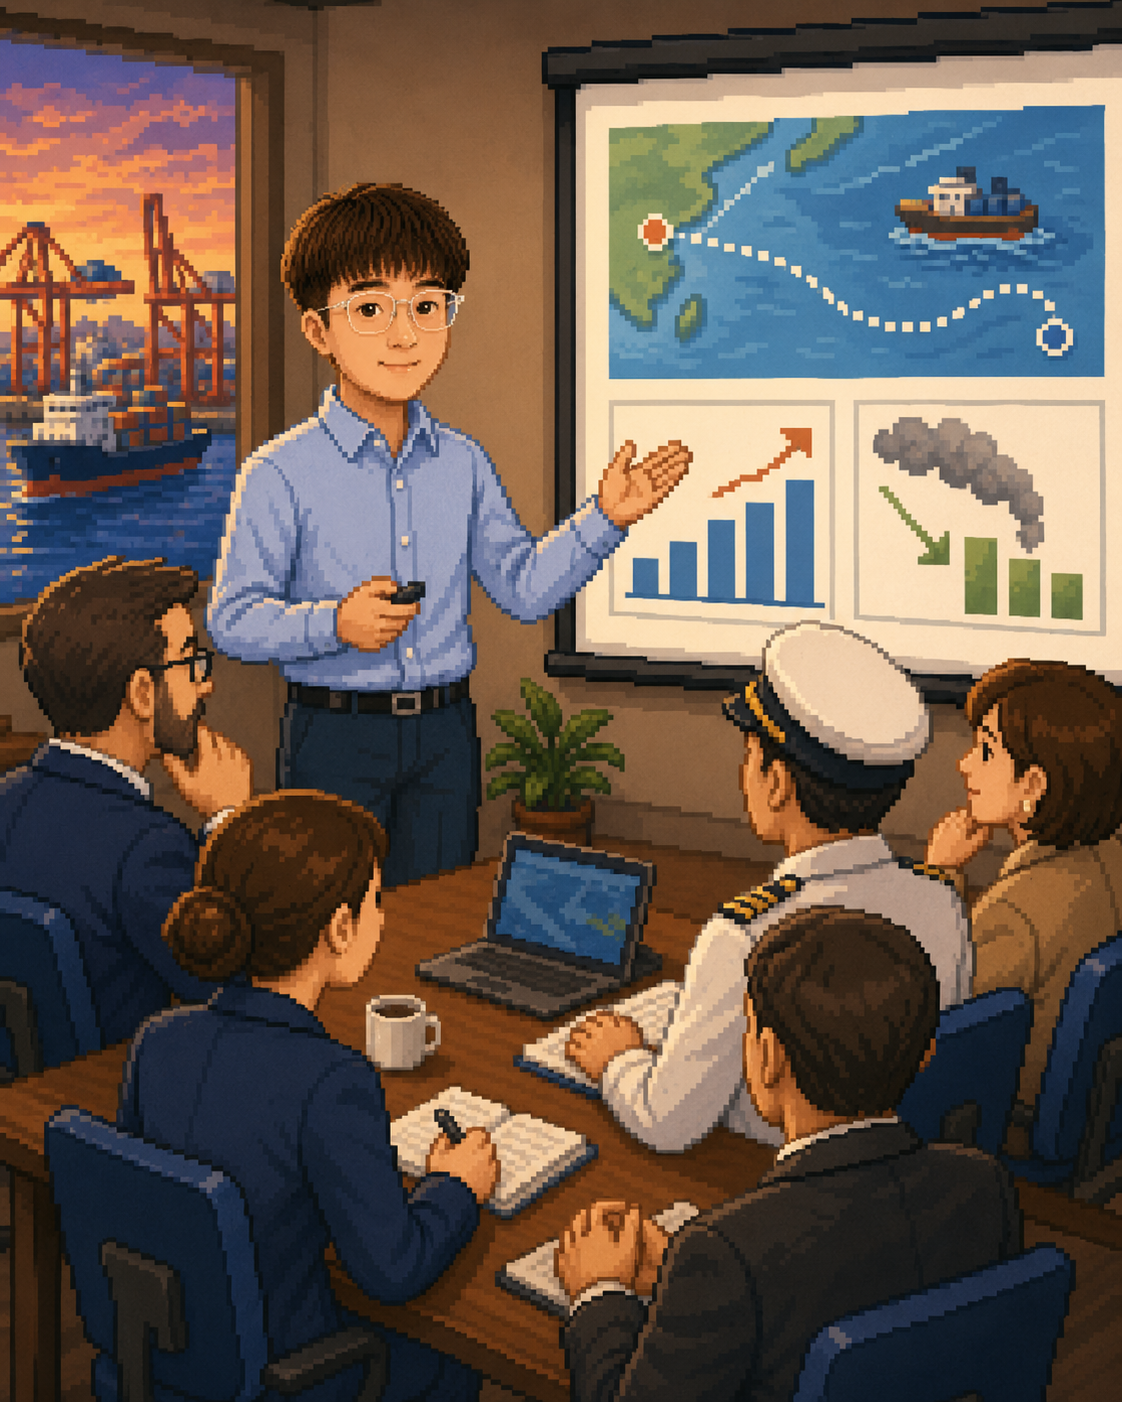
\includegraphics[
        width=0.93\linewidth,
        height=5.1cm,
        keepaspectratio
      ]{../assets/slide-10.png}
    \end{column}
  \end{columns}
  \note{
    [Sources]\par
    - Personal research framing supplied by Jeremy and his earlier
      presentation.\par
    - Visual: user-supplied illustrative stakeholder-presentation graphic,
      assets/slide-10.png.
  }
\end{frame}

% Slide 10 — sharing the research
\begin{frame}[plain]
  \begin{tikzpicture}[remember picture,overlay]
    \node[anchor=center,inner sep=0pt] at (current page.center) {%
      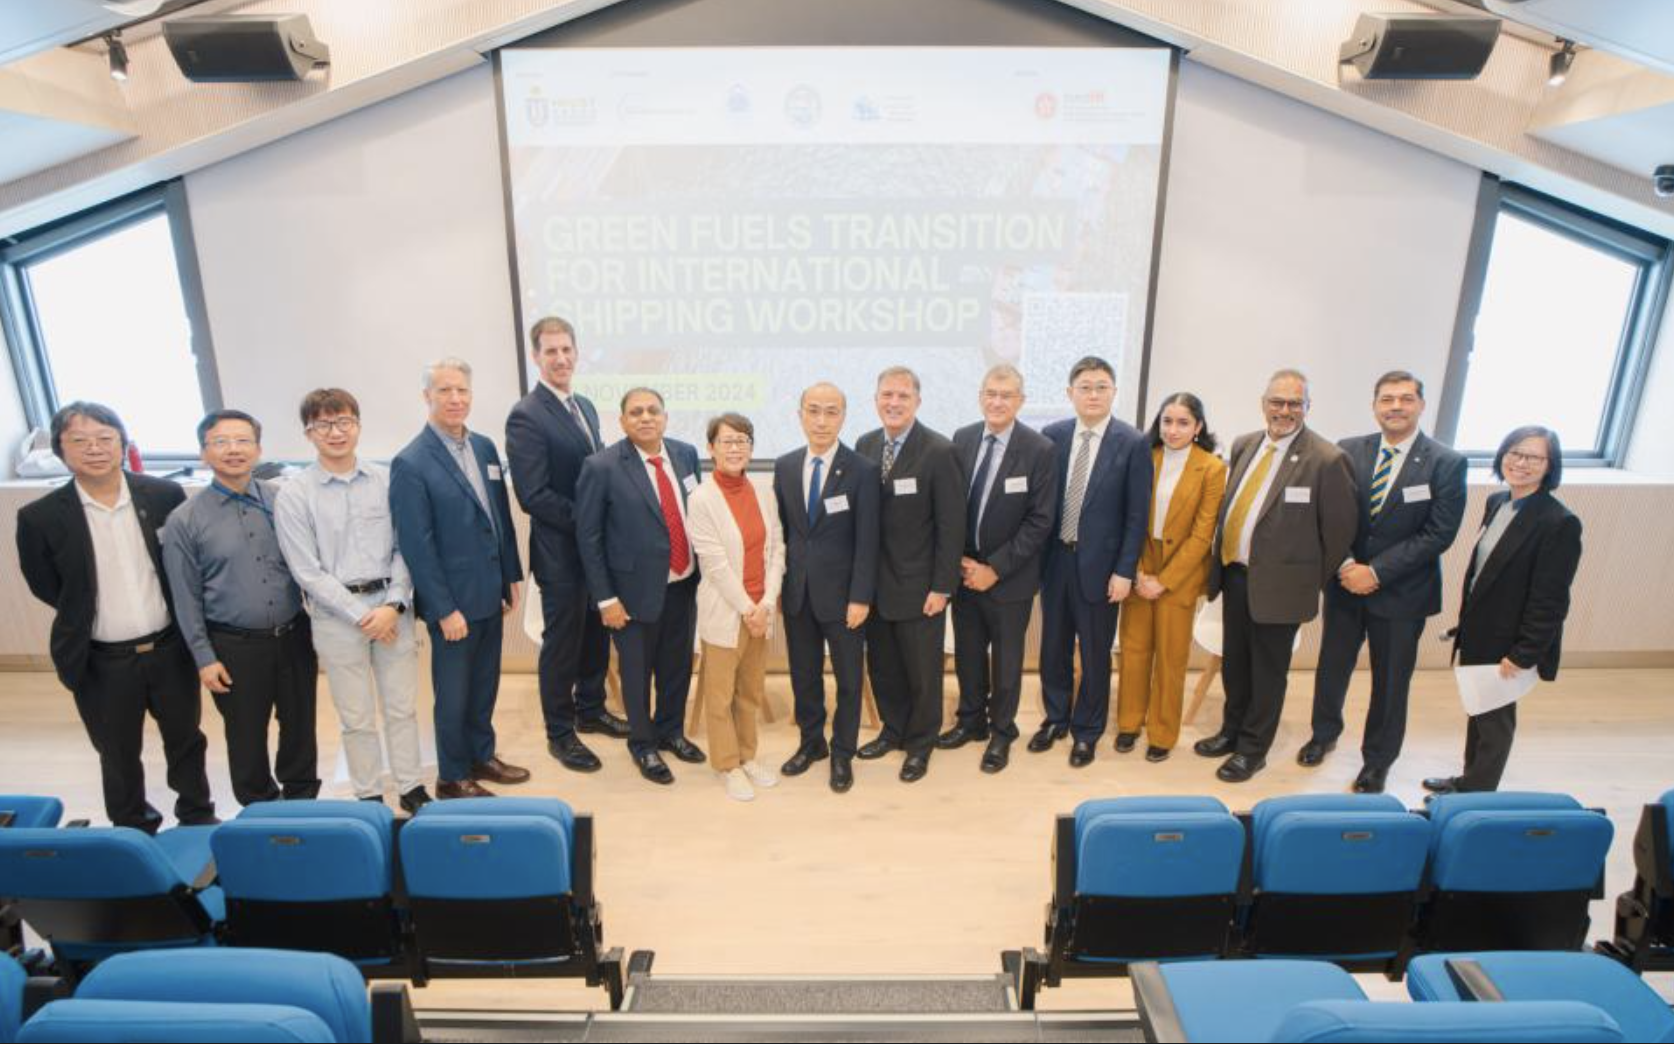
\includegraphics[
        width=\paperwidth
      ]{../assets/slide-11.png}%
    };
  \end{tikzpicture}
  \note{
    [Sources]\par
    - Personal presentation and event experience supplied by Jeremy.\par
    - Visual: user-supplied group photograph from the Green Fuels Transition
      for International Shipping Workshop, November 2024,
      assets/slide-11.png.
  }
\end{frame}

% Slide 11 — ideal post-PhD plan
\begin{frame}{The ideal plan is to stay in shipping research.}
  \vspace{0.1cm}
  \begin{columns}[T,onlytextwidth]
    \begin{column}{0.58\textwidth}
      {\color{Ink}\fontsize{13.2}{18}\selectfont
        I want to keep studying how shipping works and how it can change.
      \par}

      \vspace{0.45cm}
      {\color{Ink}\fontsize{13.2}{18}\selectfont
        Ideally, my research would influence the industry and contribute
        something useful to the wider world.
      \par}
    \end{column}

    \begin{column}{0.35\textwidth}
      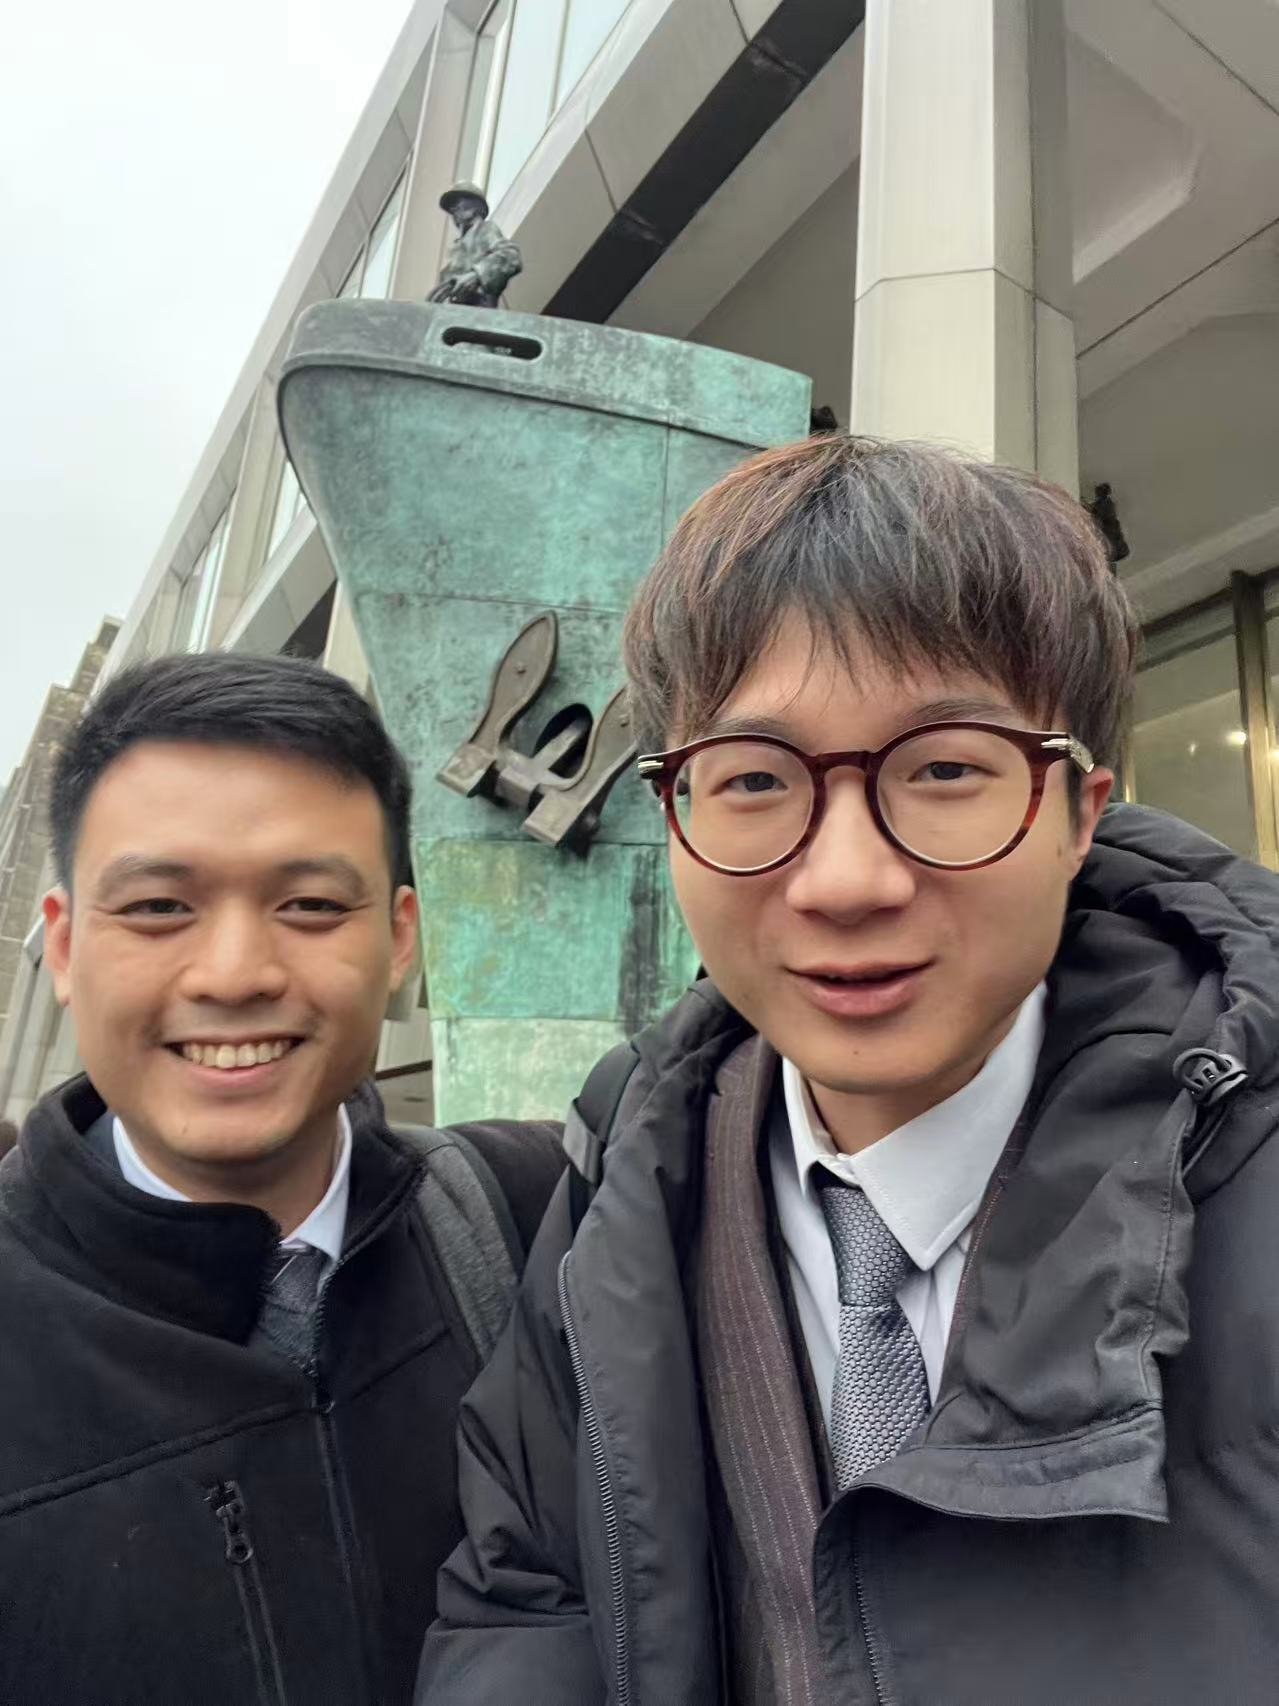
\includegraphics[
        width=0.93\linewidth,
        height=5.1cm,
        keepaspectratio
      ]{../assets/slide-12.jpg}
    \end{column}
  \end{columns}
  \note{
    [Sources]\par
    - Post-PhD ideal scenario stated directly by Jeremy.\par
    - Visual: user-supplied maritime-stakeholder photograph,
      assets/slide-12.jpg.
  }
\end{frame}

% Slide 12 — Part 1 transition
\begin{frame}[plain]
  \vfill
  \partlabel{From my story to the research}
  \vspace{0.3cm}
  {\color{Navy}\rule{1.3cm}{0.9pt}\par}

  \vspace{0.52cm}
  {\color{Ink}\fontsize{29}{34}\selectfont\bfseries
    What can science actually do\\
    for maritime decarbonisation?
  \par}

  \vspace{0.48cm}
  {\color{Ink}\fontsize{14}{18.5}\selectfont
    After the break, we will move from my journey\\
    to the practical role of evidence.
  \par}

  \vfill
  {\color{Muted}\fontsize{9.5}{12}\selectfont Part 2 begins around 11:00\par}
  \note{
    [Sources]\par
    - Transition follows the approved two-part lecture structure.
  }
\end{frame}

% Part 2 uses a quieter title scale suited to lecture content.
\setbeamerfont{frametitle}{size=\fontsize{17.28}{20.5},series=\bfseries}

% Slide 13 — opening policy question
\begin{frame}{Is shipping a significant source of global carbon emissions?}
  \vspace{0.14cm}
  {\color{Ink}\fontsize{11.8}{15.5}\selectfont
    Before looking at the evidence, which of these views do you agree with?
    \vspace{0.18cm}
    \begin{itemize}
      \setlength{\itemsep}{0.2cm}
      \item Shipping is cleaner than road transport, so its emissions are a
        lower priority.
      \item Global trade depends on ships, so strong regulation could carry
        economic costs.
      \item A fleet of more than 100,000 vessels is large enough to matter
        globally.
      \item We need an emissions estimate before deciding how strongly to
        regulate shipping.
    \end{itemize}
  }

  \note{
    [Sources]\par
    - Opening discussion prompt developed for this lecture.\par
    - Delivery: invite estimates without confirming the answer yet.\par
    - The comparisons with road transport and aviation are prompts, not
      factual claims on this slide.
  }
\end{frame}

% Slide 14 — fuel-based emissions estimate
\begin{frame}{How can we estimate carbon emissions from shipping?}
  \vspace{0.3cm}
  \partlabel{The basic calculation}
  \vspace{0.14cm}
  {\color{Ink}\fontsize{18}{22}\selectfont\bfseries
    Fuel consumption × emission factor = CO
    {\raisebox{-0.24ex}{\fontsize{11.5}{11.5}\selectfont 2}} emissions
  \par}

  \vspace{0.46cm}
  \partlabel{A simple example}
  \vspace{0.14cm}
  {\color{Ink}\fontsize{15.5}{19.5}\selectfont
    1 tonne of marine diesel × 3.206%
    {\fontsize{9}{10}\selectfont\footnotemark[1]}
    \quad≈\quad
    3.2 tonnes of CO
    {\raisebox{-0.24ex}{\fontsize{10}{10}\selectfont 2}}
  \par}
  \footnotetext[1]{The exact emission factor depends on the fuel. Around 3.2
  is a useful classroom approximation for conventional marine fuel.}

  \vfill
  {\color{Navy}\fontsize{10.5}{13.5}\selectfont\bfseries
    The next question is therefore simple: how much fuel does the fleet use?
  \par}
  \note{
    [Sources]\par
    - IMO guidance: CO2 emissions equal fuel consumption multiplied by the
      fuel-specific emission factor.\par
    - Diesel/gas oil factor: 3.206 tonnes CO2 per tonne of fuel; heavy fuel oil
      factor: 3.114.\par
    - https://gmn-phase-1.imo.org/wp-content/uploads/2019/02/PP2-Quick-guidance-printed-version.pdf
  }
\end{frame}

% Slide 15 — global fuel-use estimation
\begin{frame}{But how do we know the fuel use of every ship?}
  \vspace{0.08cm}
  {\color{Ink}\fontsize{11.2}{14.5}\selectfont
    At the start of 2026, the global merchant fleet included around
    \textbf{116,000 vessels}. We cannot collect detailed fuel records from
    every ship.
  \par}

  \vspace{0.26cm}
  \partlabel{One ship, then the whole fleet}
  \vspace{0.12cm}
  {\color{Ink}\fontsize{12}{15.5}\selectfont
    Maritime big data gives us a moving diary for each ship.
    \vspace{0.16cm}
    \begin{enumerate}
      \setlength{\itemsep}{0.14cm}
      \item See when one ship is sailing, waiting or in port.
      \item Combine its activity with ship and engine information to estimate
        fuel use.
      \item Repeat for every observed ship and add the estimates.
    \end{enumerate}
  }
  \note{
    [Sources]\par
    - UN Trade and Development data insight: around 116,000 vessels of at
      least 100 gross tons in the global merchant fleet at the start of
      2026.\par
    - https://unctadstat.unctad.org/insights/theme/243\par
    - Bottom-up explanation simplified from the Fourth IMO GHG Study
      ship-activity methodology.
  }
\end{frame}

% Slide 16 — maritime big-data teaching diagram
\begin{frame}[plain]
  \begin{tikzpicture}[remember picture,overlay]
    \node[anchor=south west,inner sep=0pt] at (current page.south west) {%
      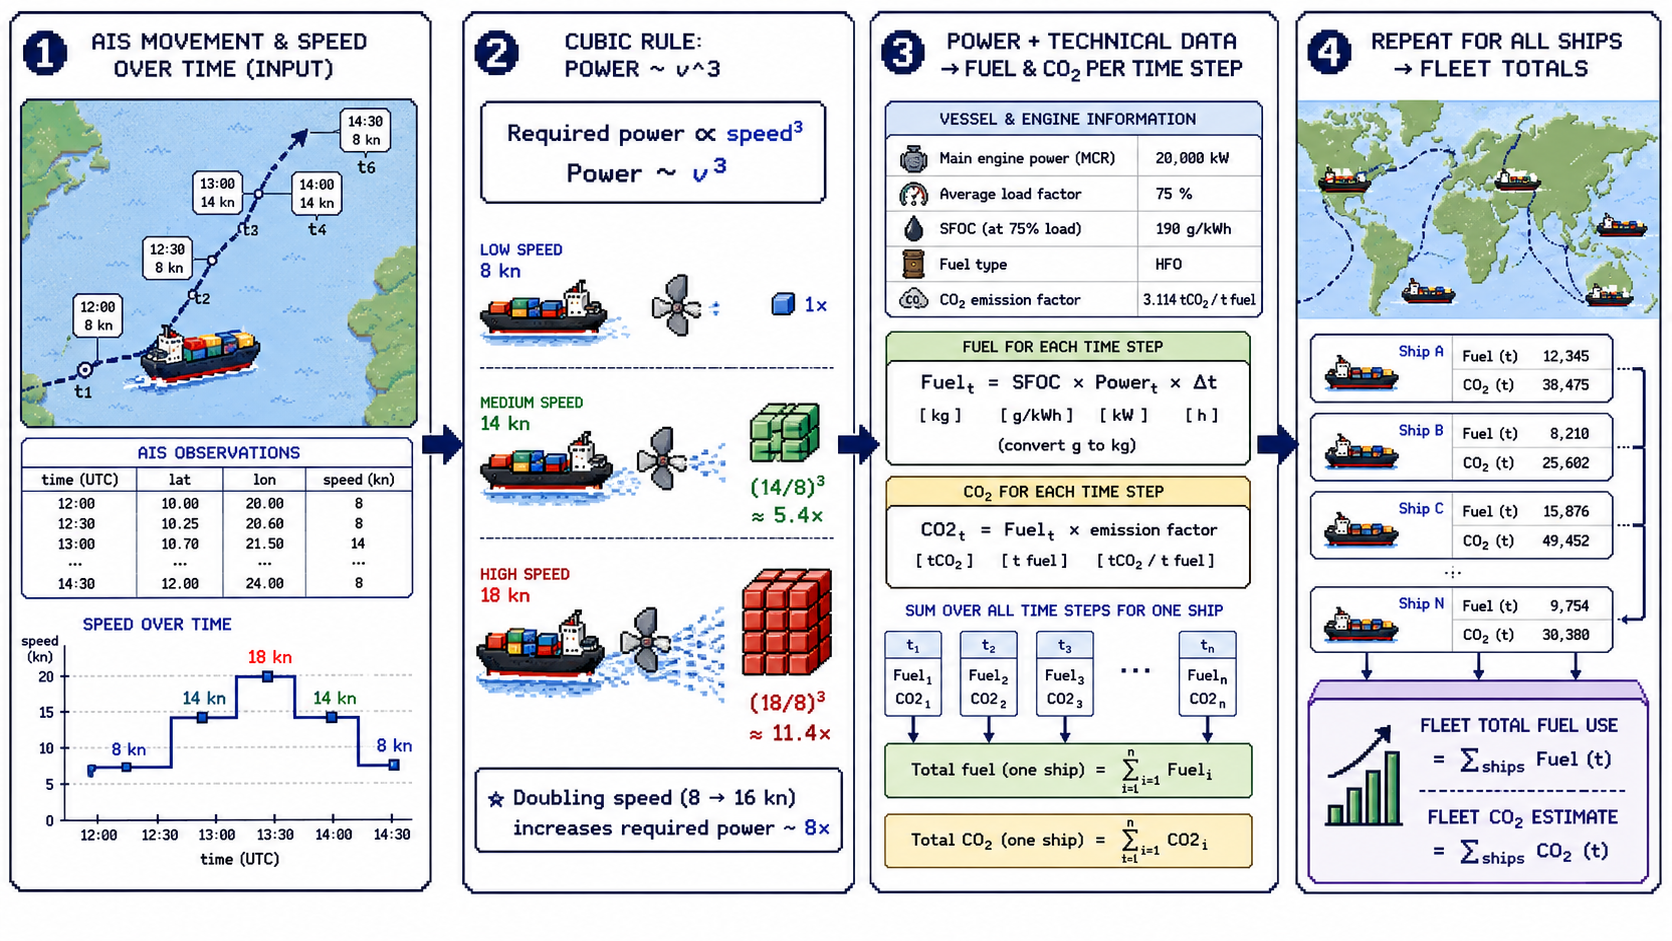
\includegraphics[
        width=\paperwidth,
        height=\paperheight,
        keepaspectratio
      ]{../assets/slide-17.png}%
    };
  \end{tikzpicture}
  \note{
    [Sources]\par
    - Visual brief developed from Jeremy's explanation of maritime big data
      and the bottom-up method.\par
    - Visual: user-supplied illustrative teaching diagram,
      assets/slide-17.png.
  }
\end{frame}

% Slide 17 — IMO evidence
\begin{frame}{A global study provides the evidence}
  \vspace{0.04cm}
  {\color{Ink}\fontsize{10.8}{14}\selectfont
    The Fourth International Maritime Organization (IMO) Greenhouse Gas Study
    estimated that total shipping emitted in 2018:
  \par}

  \vspace{0.28cm}
  \begin{columns}[c,onlytextwidth]
    \begin{column}{0.54\textwidth}
      {\color{Ink}\fontsize{29}{33}\selectfont\bfseries
        1,056 million\\
        tonnes
      \par}
      \vspace{0.08cm}
      {\color{Muted}\fontsize{10.5}{13.5}\selectfont
        of CO{\raisebox{-0.24ex}{\fontsize{7}{7}\selectfont 2}}
      \par}
    \end{column}

    \begin{column}{0.06\textwidth}
      \centering
      {\color{RuleGray}\rule{0.6pt}{2.2cm}}
    \end{column}

    \begin{column}{0.34\textwidth}
      {\color{Navy}\fontsize{29}{33}\selectfont\bfseries
        2.89\%
      \par}
      \vspace{0.08cm}
      {\color{Muted}\fontsize{10.5}{13.5}\selectfont
        of global human-caused
        CO{\raisebox{-0.24ex}{\fontsize{7}{7}\selectfont 2}} emissions
      \par}
    \end{column}
  \end{columns}

  \vfill
  {\setlength{\fboxsep}{5pt}%
    \colorbox{HighlightYellow}{%
      {\color{Ink}\fontsize{10.5}{13}\selectfont\bfseries
        Science role 1: provide evidence for policy discussion}%
    }\par}
  \note{
    [Sources]\par
    - International Maritime Organization, Fourth IMO Greenhouse Gas Study
      2020: 1,056 million tonnes of CO2 in 2018 and 2.89\% of global
      anthropogenic CO2.\par
    - Scope: international, domestic and fishing vessels.\par
    - https://www.imo.org/en/ourwork/environment/pages/fourth-imo-greenhouse-gas-study-2020.aspx
  }
\end{frame}

% Slide 18 — compare pathways
\begin{frame}{There is no single decarbonisation pathway}
  \vspace{0.12cm}
  {\color{Ink}\fontsize{11.7}{15.2}\selectfont
    A transition can combine four kinds of action:
    \vspace{0.18cm}
    \begin{enumerate}
      \setlength{\itemsep}{0.19cm}
      \item \textbf{Use less energy.} Improve hulls, engines and onboard
        systems.
      \item \textbf{Operate ships differently.} Adjust speed, routing,
        loading and port calls.
      \item \colorbox{HighlightYellow}{\textbf{Change the energy source.}}
        Use fuels with lower lifecycle greenhouse gas emissions.
      \item \textbf{Prepare ports.} Provide bunkering, shore power, safety
        systems and supporting logistics.
    \end{enumerate}
  }

  \vfill
  {\color{Navy}\fontsize{10.5}{13.5}\selectfont\bfseries
    The appropriate combination depends on the ship, route, cargo and
    timescale.
  \par}
  \note{
    [Sources]\par
    - IMO 2023 GHG Strategy and Future Fuels and Technology Project.\par
    - https://www.imo.org/en/ourwork/environment/pages/imo-strategy-on-reduction-of-ghg-emissions-from-ships.aspx\par
    - https://www.imo.org/en/mediacentre/pressbriefings/pages/future-fuels-and-technology.aspx
  }
\end{frame}

% Slide 19 — implementation conditions
\begin{frame}{Implementation depends on the wider system}
  \vspace{0.12cm}
  {\color{Ink}\fontsize{11.7}{15.2}\selectfont
    A promising technology still has to pass three practical tests:
    \vspace{0.2cm}
    \begin{enumerate}
      \setlength{\itemsep}{0.24cm}
      \item \textbf{Can it work?}\\
        Are compatible vessels, fuels and port infrastructure available?
      \item \textbf{Can it pay?}\\
        Can cargo demand, finance and long-term commitments support the cost?
      \item \textbf{Can it operate within the rules?}\\
        Do safety standards and public policy enable implementation?
    \end{enumerate}
  }

  \vfill
  {\color{Navy}\fontsize{10.2}{13.2}\selectfont\bfseries
    The transition succeeds when these conditions develop together.
  \par}
  \note{
    [Sources]\par
    - Barrier categories synthesised from the IMO 2023 GHG Strategy and the
      Clydebank Declaration's focus on partnerships, regulation, incentives,
      information and infrastructure.\par
    - https://www.gov.uk/government/publications/cop-26-clydebank-declaration-for-green-shipping-corridors/cop-26-clydebank-declaration-for-green-shipping-corridors
  }
\end{frame}

% Slide 20 — Green Shipping Corridors and coordination
\begin{frame}{Green Shipping Corridors coordinate action}
  \vspace{0.08cm}
  \begin{columns}[T,onlytextwidth]
    \begin{column}{0.58\textwidth}
      {\color{Ink}\fontsize{11.4}{14.8}\selectfont
        A Green Shipping Corridor is a route between two or more ports where
        partners work together to advance zero-emission shipping.
        \vspace{0.18cm}
        \begin{itemize}
          \setlength{\itemsep}{0.11cm}
          \item Start with one route and an existing shipping service.
          \item Bring cargo owners, ship operators, ports and fuel providers
            into the same process.
          \item Align vessels, fuel, infrastructure, finance, standards and
            policy.
        \end{itemize}
      }
    \end{column}

    \begin{column}{0.35\textwidth}
      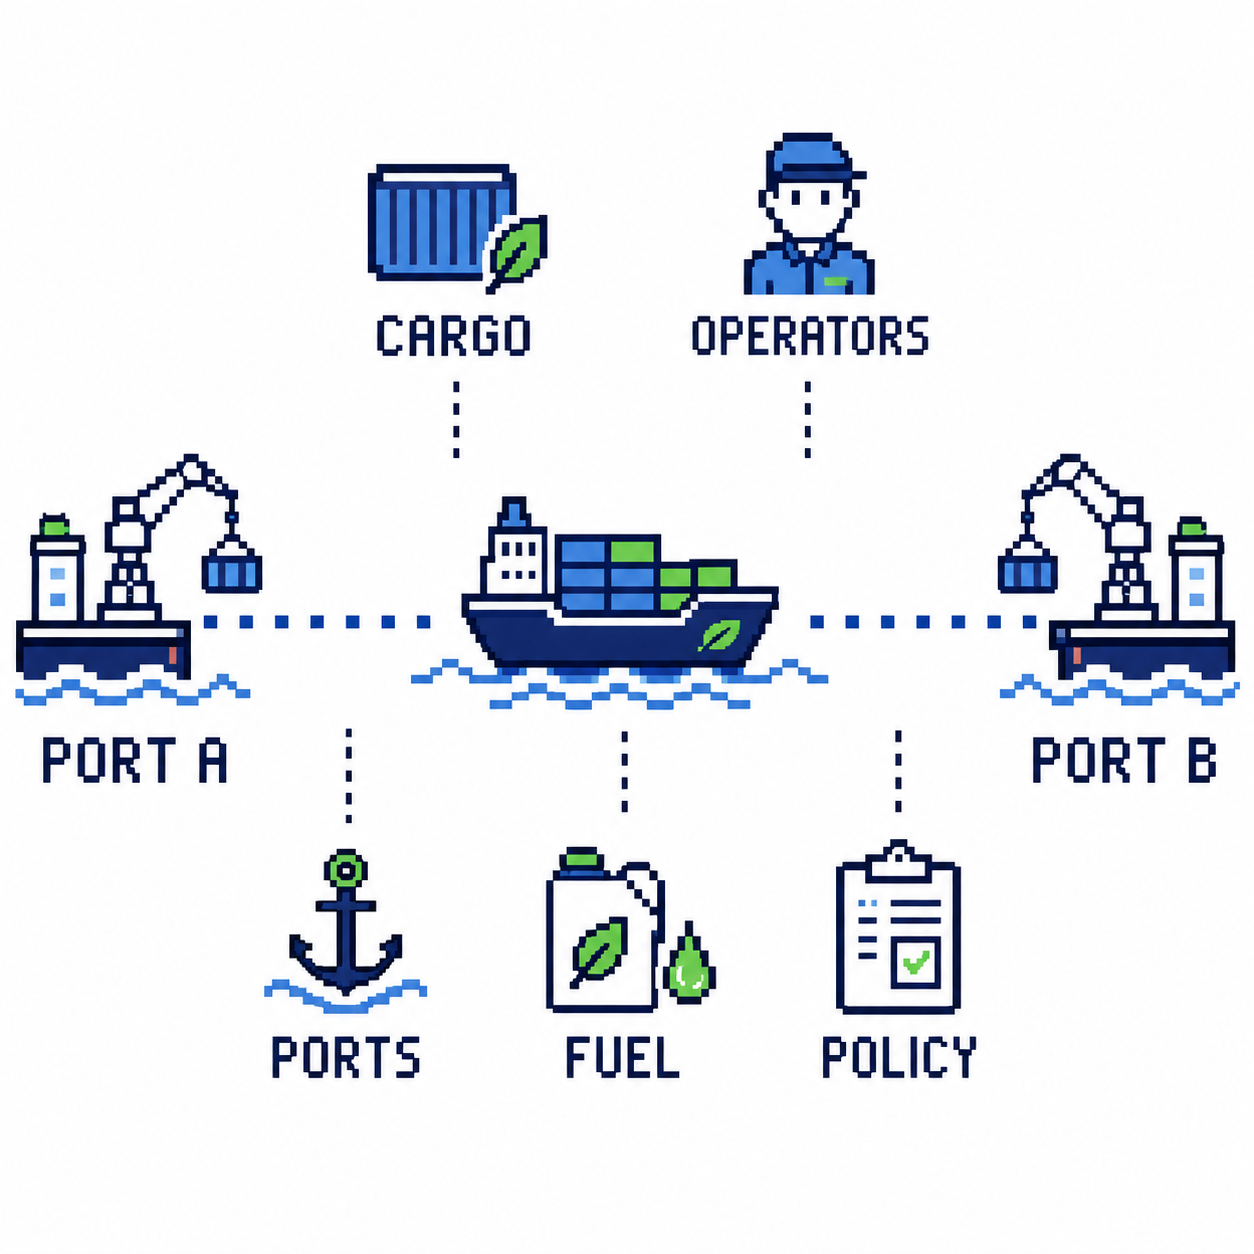
\includegraphics[
        width=0.93\linewidth,
        height=5.1cm,
        keepaspectratio
      ]{../assets/slide-21.png}
    \end{column}
  \end{columns}
  \note{
    [Sources]\par
    - Clydebank Declaration: green shipping corridors are zero-emission
      maritime routes between two or more ports, supported by partnerships
      across the value chain.\par
    - https://www.gov.uk/government/publications/cop-26-clydebank-declaration-for-green-shipping-corridors/cop-26-clydebank-declaration-for-green-shipping-corridors\par
    - Optional prompt: is a corridor a route, a technology or a coordination
      mechanism? Answer: primarily a coordination mechanism focused on a
      route.\par
    - Visual: user-supplied illustrative coordination graphic,
      assets/slide-21.png.
  }
\end{frame}

% Slide 21 — Green Shipping Corridor implementation dilemma
\begin{frame}{The idea is attractive. Delivery is difficult.}
  \vspace{0.04cm}
  {\color{Ink}\fontsize{10.8}{14}\selectfont
    The 2025 global progress review tracked:
  \par}

  \vspace{0.28cm}
  \begin{columns}[c,onlytextwidth]
    \begin{column}{0.47\textwidth}
      {\color{Ink}\fontsize{31}{35}\selectfont\bfseries 84\par}
      \vspace{0.06cm}
      {\color{Muted}\fontsize{10.3}{13.2}\selectfont
        active Green Shipping Corridor initiatives
      \par}
    \end{column}

    \begin{column}{0.06\textwidth}
      \centering
      {\color{RuleGray}\rule{0.6pt}{1.9cm}}
    \end{column}

    \begin{column}{0.41\textwidth}
      {\color{Navy}\fontsize{31}{35}\selectfont\bfseries 4\par}
      \vspace{0.06cm}
      {\color{Muted}\fontsize{10.3}{13.2}\selectfont
        had reached the realisation stage
      \par}
    \end{column}
  \end{columns}

  \vspace{0.3cm}
  {\setlength{\fboxsep}{4pt}%
    \colorbox{HighlightYellow}{%
      {\color{Ink}\fontsize{10.5}{13}\selectfont\bfseries
        The feasibility wall}%
    }\par}
  \vspace{0.12cm}
  {\color{Ink}\fontsize{11.2}{14.5}\selectfont
    Many initiatives remain stalled because zero-emission fuels still cost
    more than conventional fuels.
  \par}

  \vfill
  {\color{Navy}\fontsize{10.2}{13.2}\selectfont\bfseries
    Which routes have the strongest starting conditions?
  \par}
  \vspace{0.08cm}
  {\color{Muted}\fontsize{8.2}{10.2}\selectfont
    Source: Global Maritime Forum, Annual Progress Report on Green Shipping
    Corridors 2025.
  \par}
  \note{
    [Sources]\par
    - Global Maritime Forum, Annual Progress Report on Green Shipping
      Corridors 2025: 84 active initiatives, four at the realisation stage and
      many initiatives facing a feasibility wall associated with the cost gap
      between conventional and zero-emission fuels.\par
    - https://globalmaritimeforum.org/report/annual-progress-report-on-green-shipping-corridors-2025/
  }
\end{frame}

% Slide 22 — maritime data and route selection
\begin{frame}{Maritime big data helps identify promising corridors}
  \vspace{0.05cm}
  {\color{Ink}\fontsize{10.8}{14}\selectfont
    The same movement data used to estimate emissions can reveal which routes
    have the strongest starting conditions.
  \par}

  \vspace{0.18cm}
  \begin{columns}[T,onlytextwidth]
    \begin{column}{0.58\textwidth}
      {\color{Ink}\fontsize{10.9}{14.2}\selectfont
        \begin{enumerate}
          \setlength{\itemsep}{0.14cm}
          \item Find routes with regular, repeated movement between ports.
          \item Identify the vessels and operators already serving each route.
          \item Compare traffic scale and service concentration across
            candidate routes.
        \end{enumerate}
      }
    \end{column}

    \begin{column}{0.35\textwidth}
      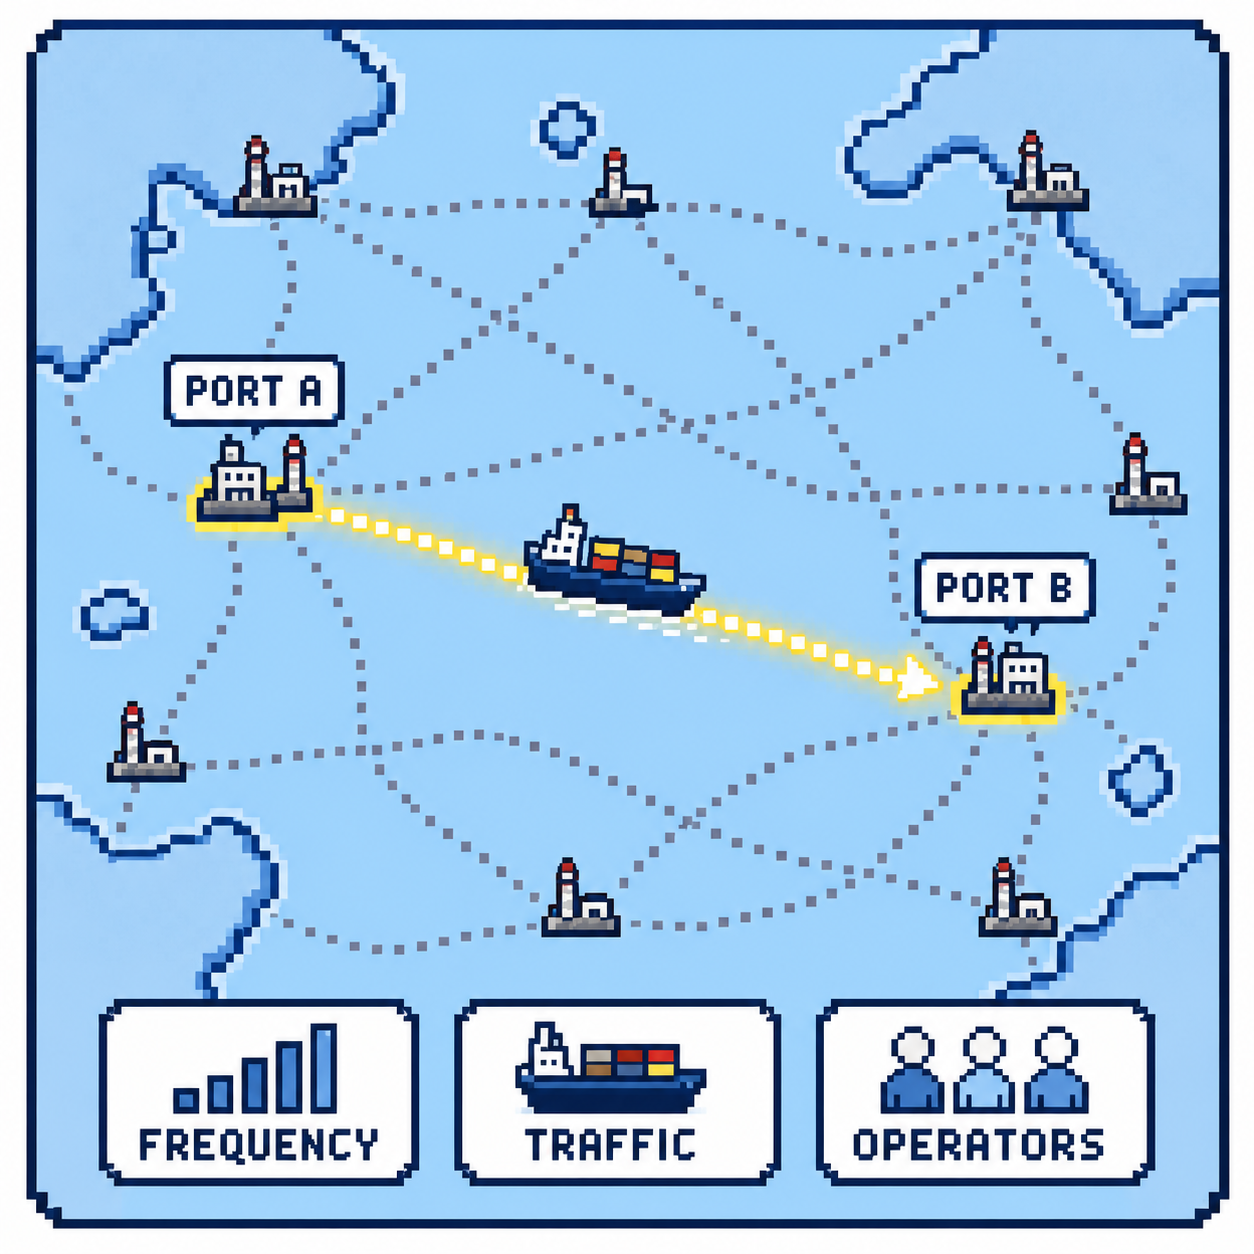
\includegraphics[
        width=0.93\linewidth,
        height=3.85cm,
        keepaspectratio
      ]{../assets/slide-23.png}
    \end{column}
  \end{columns}
  \vfill
  {\setlength{\fboxsep}{4pt}%
    \colorbox{HighlightYellow}{%
      {\color{Ink}\fontsize{9.8}{12.3}\selectfont\bfseries
        Science role 2: identify routes with a credible starting point}%
    }\par}
  \note{
    [Sources]\par
    - Research framing supplied by Jeremy and adapted from the approved Green
      Shipping Corridor case.\par
    - Global Maritime Forum: some trade routes offer relative advantages
      because of fuel access, operational profiles or economics; corridors
      seek to identify and leverage those routes.\par
    - https://globalmaritimeforum.org/green-corridors/\par
    - Visual: user-supplied illustrative candidate-route map,
      assets/slide-23.png.
  }
\end{frame}

% Slide 23 — why the Hong Kong–San Antonio route stands out
\begin{frame}{Why San Antonio--Hong Kong stands out}
  \vspace{0.08cm}
  \partlabel{2021 route analysis · \#1 by estimated fuel demand}

  \vspace{0.3cm}
  \begin{columns}[T,onlytextwidth]
    \begin{column}{0.22\textwidth}
      {\color{Navy}\fontsize{25}{28}\selectfont\bfseries 52\par}
      \vspace{0.05cm}
      {\color{Muted}\fontsize{9.5}{12}\selectfont
        two-way voyages
      \par}
    \end{column}

    \begin{column}{0.22\textwidth}
      {\color{Navy}\fontsize{25}{28}\selectfont\bfseries 29\par}
      \vspace{0.05cm}
      {\color{Muted}\fontsize{9.5}{12}\selectfont
        ships serving the route
      \par}
    \end{column}

    \begin{column}{0.22\textwidth}
      {\color{Navy}\fontsize{25}{28}\selectfont\bfseries 23.3\par}
      \vspace{0.05cm}
      {\color{Muted}\fontsize{9.5}{12}\selectfont
        average voyage days
      \par}
    \end{column}

    \begin{column}{0.25\textwidth}
      {\color{Navy}\fontsize{22}{25}\selectfont\bfseries 243,725\par}
      \vspace{0.05cm}
      {\color{Muted}\fontsize{9.5}{12}\selectfont
        tonnes of estimated annual fuel demand
      \par}
    \end{column}
  \end{columns}

  \vspace{0.42cm}
  {\color{RuleGray}\rule{\textwidth}{0.5pt}\par}

  \vfill
  {\setlength{\fboxsep}{4pt}%
    {\color{Ink}\fontsize{10.1}{13.2}\selectfont
      \textbf{Why it matters:} regular, long-haul traffic creates
      \colorbox{HighlightYellow}{\textbf{predictable fuel demand}} and a
      meaningful opportunity for cleaner fuels.
    \par}}
  \note{
    [Sources]\par
    - Jeremy's April 2025 presentation: 2021 two-way route analysis ranked
      San Antonio--Hong Kong first among candidate corridors by estimated fuel
      demand; 52 voyages, 29 ships, 23.3 average voyage days and 243,725
      tonnes of estimated annual fuel demand.\par
    - Jeremy's op-ed, Cherries to Carbon: the scale and regularity of this
      long-haul traffic create predictable fuel demand and a meaningful
      opportunity for emissions reduction through cleaner fuels.\par
    - Visual: no external image; the slide uses a native four-metric layout.
  }
\end{frame}

% Slide 24 — research into policy dialogue
\begin{frame}{Research can inform policy dialogue}
  \vspace{0.02cm}
  \begin{columns}[T,onlytextwidth]
    \begin{column}{0.58\textwidth}
      {\setlength{\fboxsep}{4pt}%
        \colorbox{HighlightYellow}{%
          {\color{Ink}\fontsize{9.2}{11.2}\selectfont\bfseries April 2025}%
        }\par}
      \vspace{0.12cm}
      {\color{Ink}\fontsize{11.8}{15.5}\selectfont
        I presented evidence on the route and its potential as a Green
        Shipping Corridor.
      \par}

      \vspace{0.18cm}
      {\setlength{\fboxsep}{4pt}%
        \colorbox{HighlightYellow}{%
          {\color{Ink}\fontsize{9.2}{11.2}\selectfont\bfseries
            17 November 2025}%
        }\par}
      \vspace{0.12cm}
      {\color{Ink}\fontsize{11.8}{15.5}\selectfont
        San Antonio was announced among Hong Kong’s first Partner Ports.
      \par}

      \vspace{0.18cm}
      \partlabel{Continuing work}
      \vspace{0.12cm}
      {\color{Ink}\fontsize{11.8}{15.5}\selectfont
        Research, stakeholder dialogue and practical coordination continue.
      \par}
    \end{column}

    \begin{column}{0.35\textwidth}
      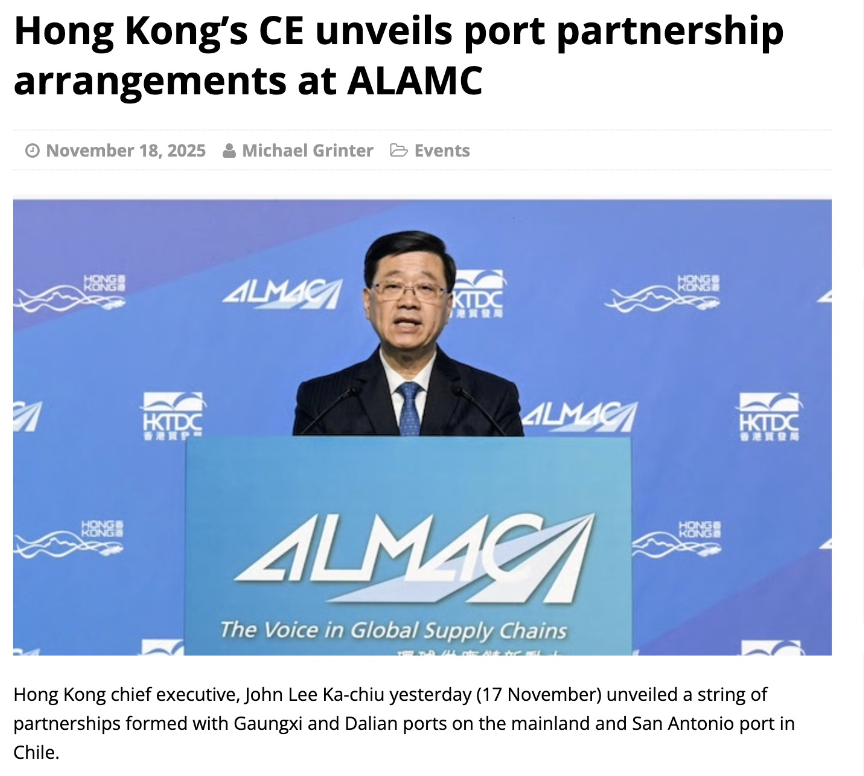
\includegraphics[
        width=0.93\linewidth,
        height=5.1cm,
        keepaspectratio
      ]{../assets/slide-25.png}
    \end{column}
  \end{columns}
  \note{
    [Sources]\par
    - April 2025 presentation: Jeremy's personal account and presentation
      record supplied privately.\par
    - Hong Kong Transport and Logistics Bureau, 17 November 2025: San Antonio
      Port of Chile was included in the first batch of Partner Ports.\par
    - https://www.tlb.gov.hk/eng/psp/pressreleases/transport/2025/20251117c.html\par
    - Delivery note: present this as a sequence and contribution to dialogue,
      not as proof that the research caused the Partner Port decision.\par
    - Visual: user-supplied screenshot of Hong Kong Maritime Hub, Hong Kong's
      CE unveils port partnership arrangements at ALAMC, 18 November 2025,
      assets/slide-25.png.
  }
\end{frame}

% Slide 25 — conclusion
\begin{frame}{What science contributes}
  \vspace{0.15cm}
  {\color{Ink}\fontsize{12}{15.7}\selectfont
    \begin{itemize}
      \setlength{\itemsep}{0.18cm}
      \item A more reliable understanding of the emissions problem.
      \item A transparent basis for comparing possible pathways.
      \item Evidence on feasibility, uncertainty and trade-offs.
      \item A shared analytical foundation for coordination.
    \end{itemize}
  }

  \vspace{0.3cm}
  {\color{Navy}\rule{\textwidth}{0.65pt}\par}
  \vspace{0.25cm}
  {\color{Ink}\fontsize{12.2}{16}\selectfont\bfseries
    Policy decisions also reflect institutions, economics, politics and
    values.
  \par}

  \vfill
  \note{
    [Sources]\par
    - Closing synthesis follows the approved lecture argument and the IMO
      2023 GHG Strategy's recognition of technical, institutional and
      supportive measures.
  }
\end{frame}

% Slide 26 — thank you and contact
\begin{frame}[plain]
  \begin{tikzpicture}[remember picture,overlay]
    \node[anchor=center,inner sep=0pt] at (current page.center) {%
      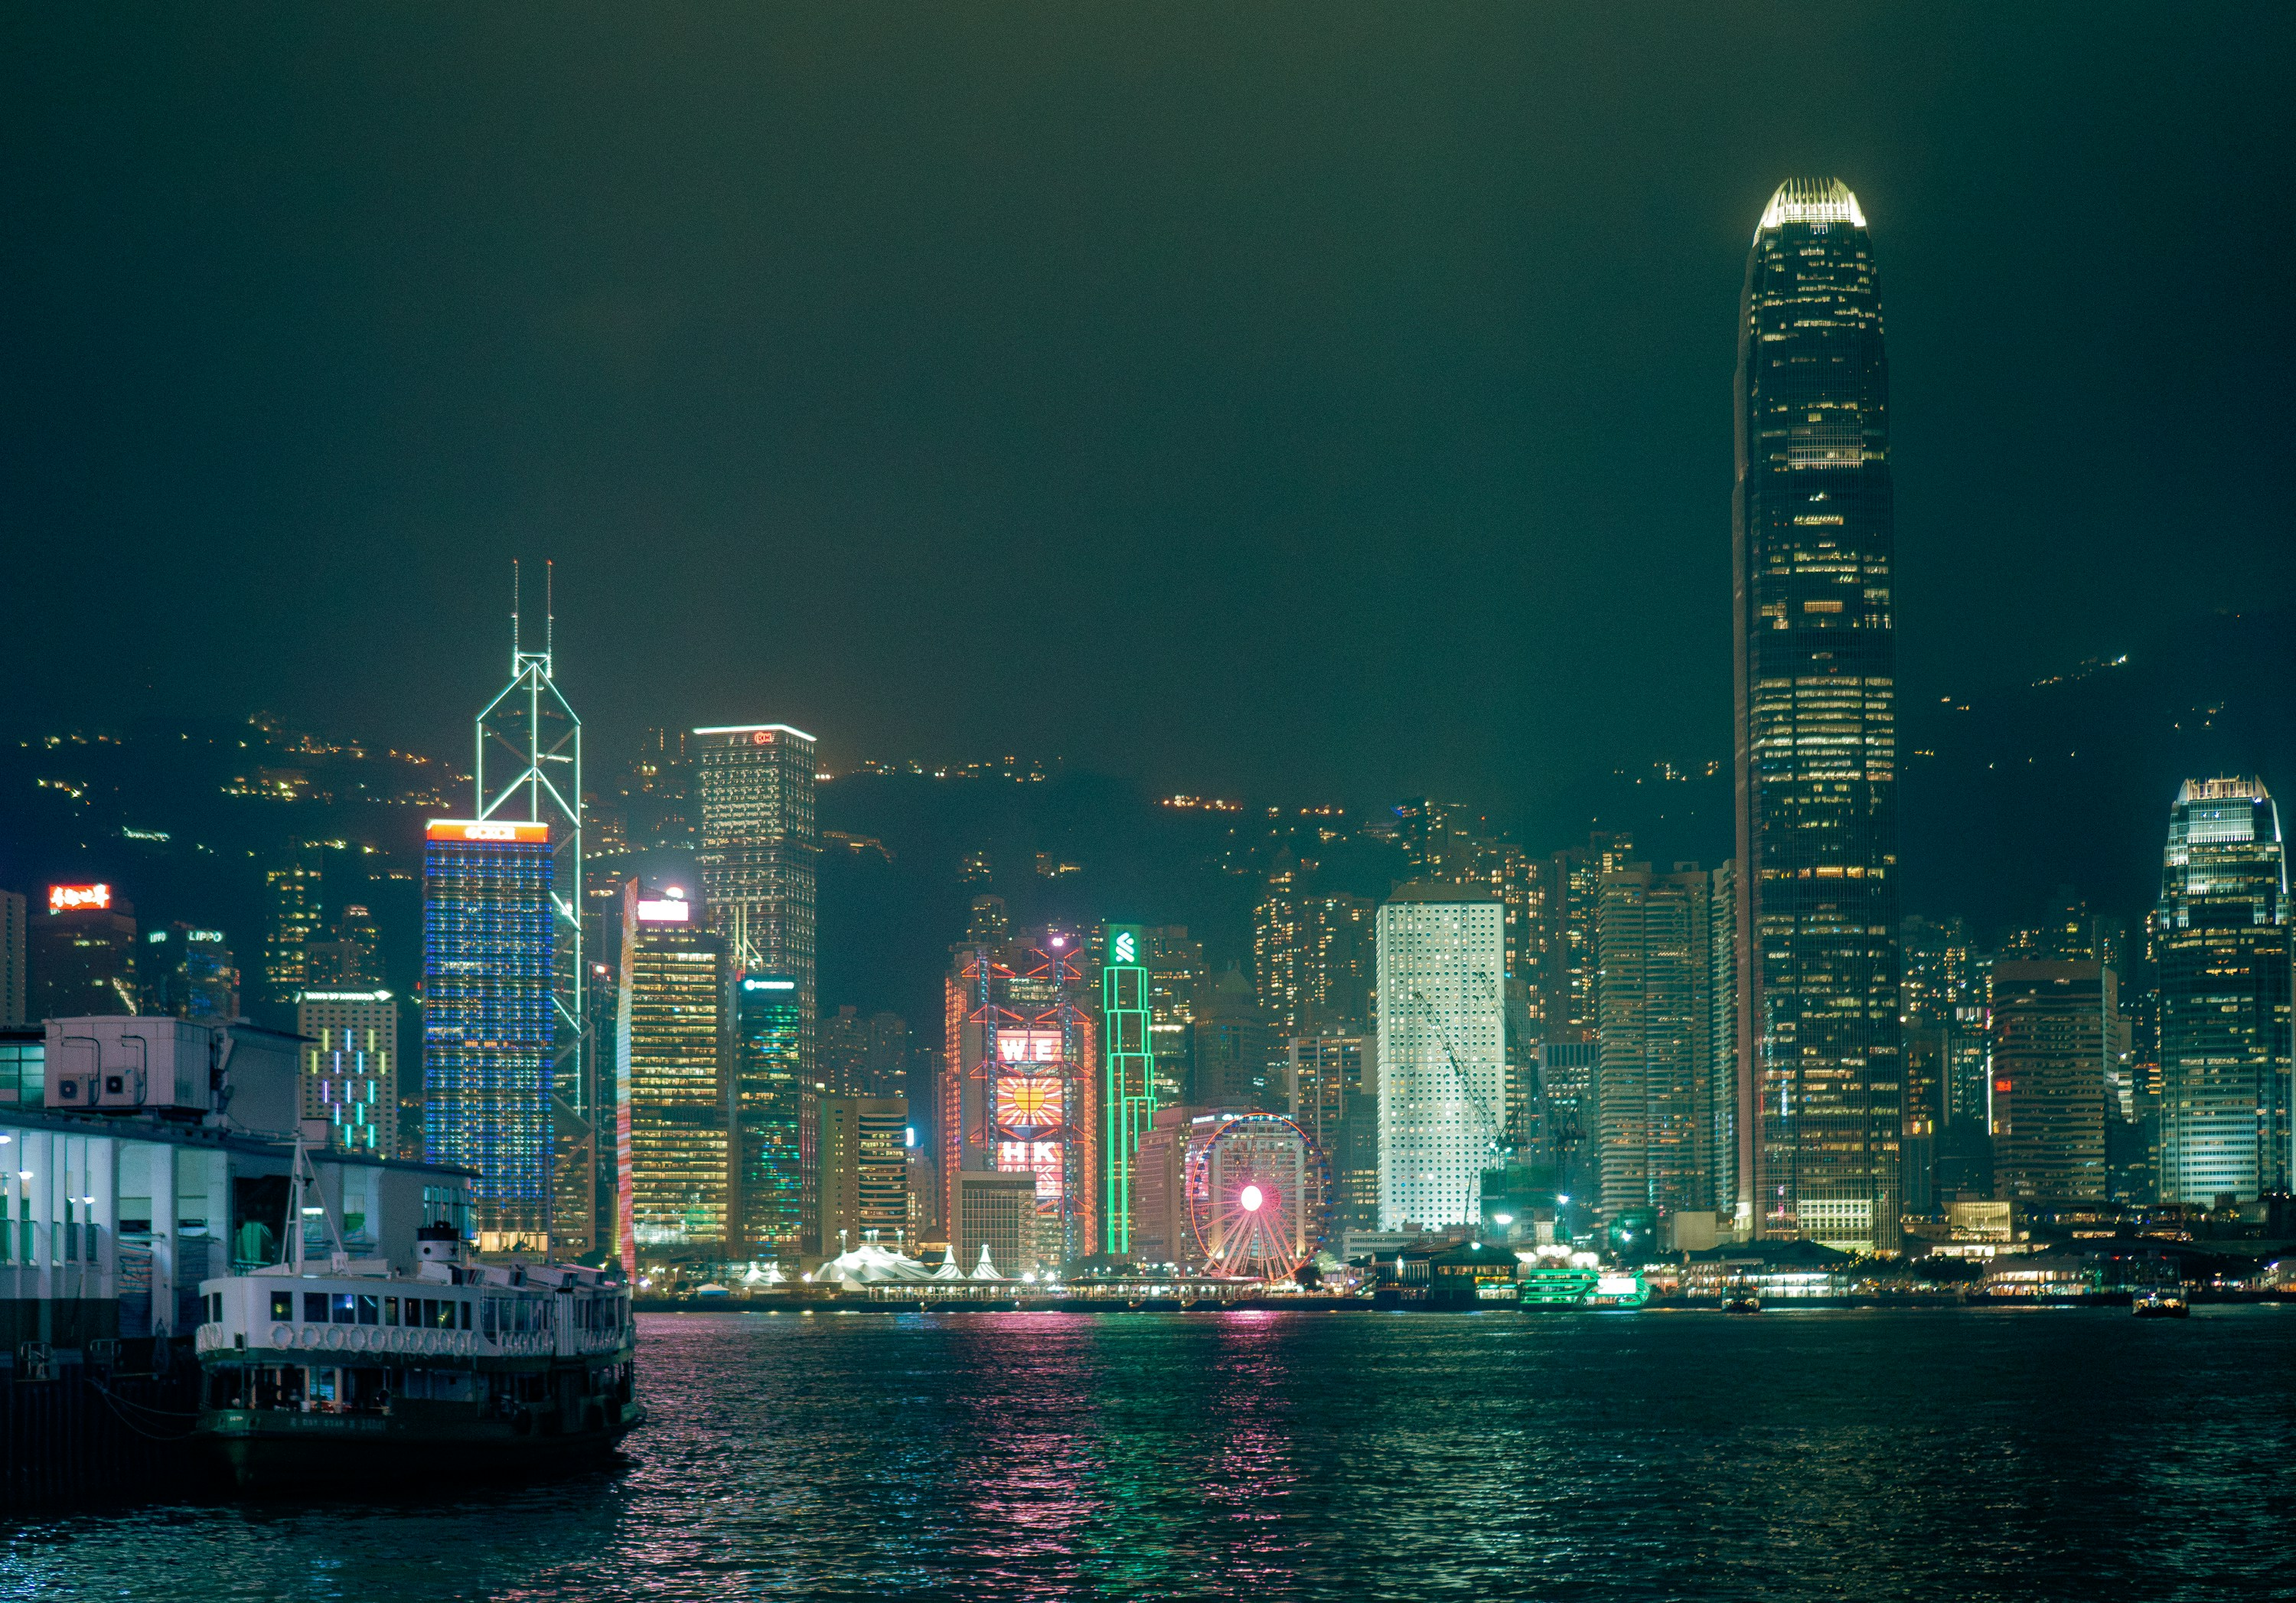
\includegraphics[
        trim=0 203bp 0 203bp,
        clip,
        width=\paperwidth
      ]{../assets/hong-kong-victoria-harbour-raymond-yeung.jpg}%
    };
    \fill[black,opacity=0.58]
      (current page.south west) rectangle (current page.north east);
  \end{tikzpicture}

  \vfill
  {\color{white}\fontsize{9}{11}\selectfont\bfseries THANK YOU\par}
  \vspace{0.3cm}
  {\color{white}\rule{1.3cm}{0.9pt}\par}

  \vspace{0.5cm}
  {\color{white}\fontsize{30}{34}\selectfont\bfseries
    Questions?
  \par}

  \vspace{0.52cm}
  {\color{white}\fontsize{13}{17}\selectfont\bfseries
    Jeremy Jiajing Chen
  \par}
  \vspace{0.18cm}
  {\color{white}\fontsize{11.5}{15}\selectfont
    Email:\enspace
    \href{mailto:jchenhl@connect.ust.hk}{%
      \textcolor{white}{jchenhl@connect.ust.hk}}
  \par}
  \vspace{0.1cm}
  {\color{white}\fontsize{11.5}{15}\selectfont
    Website:\enspace
    \href{https://amoylimee.github.io/}{%
      \textcolor{white}{https://amoylimee.github.io/}}
  \par}

  \vfill
  \hfill
  {\color{white}\fontsize{6.8}{8.2}\selectfont
    Photo: Raymond Yeung / Unsplash
  \par}
  \note{
    [Sources]\par
    - Contact email and personal-homepage URL supplied and approved for public
      display by Jeremy.\par
    - Hong Kong Victoria Harbour night photograph by Raymond Yeung, used under
      the Unsplash License.\par
    - https://unsplash.com/photos/nighttime-skyline-of-hong-kong-lit-up-cZ2PwQJ8Fpw
  }
\end{frame}

\end{document}
